\subsection{Meshing examples}
\paragraph{}
In this section, some other mesh examples with irregular geometric boundaries are considered.
% Fig.~\ref{} and Fig.~\ref{qdt_ex:mesh_wolli_logo} show the mesh generated for a flower input.
% Fig.~\ref{} and Fig.~\ref{qdt_ex:mesh_wolli_logo_sharp} highlight the sharp corner treatment of the algorithm.

\begin{figure}
    \centering
    \scalebox{0.25}{
        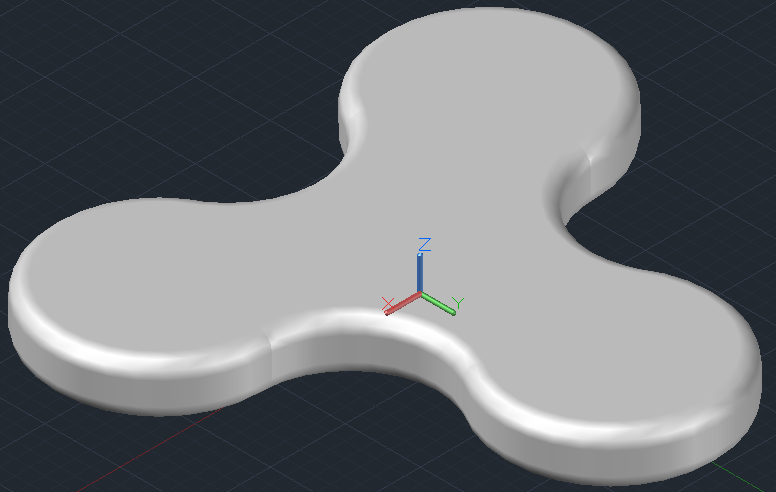
\includegraphics{octree/ex_images/spinner_cad.png}
    }
    \caption[CAD design for spinner]{CAD design for spinner}
    \label{oct_ex:mesh_spinner_cad}
\end{figure}

\begin{figure}
    \centering
    \begin{subfigure}[b]{0.49\linewidth}
        \centering
        \scalebox{0.25}{
            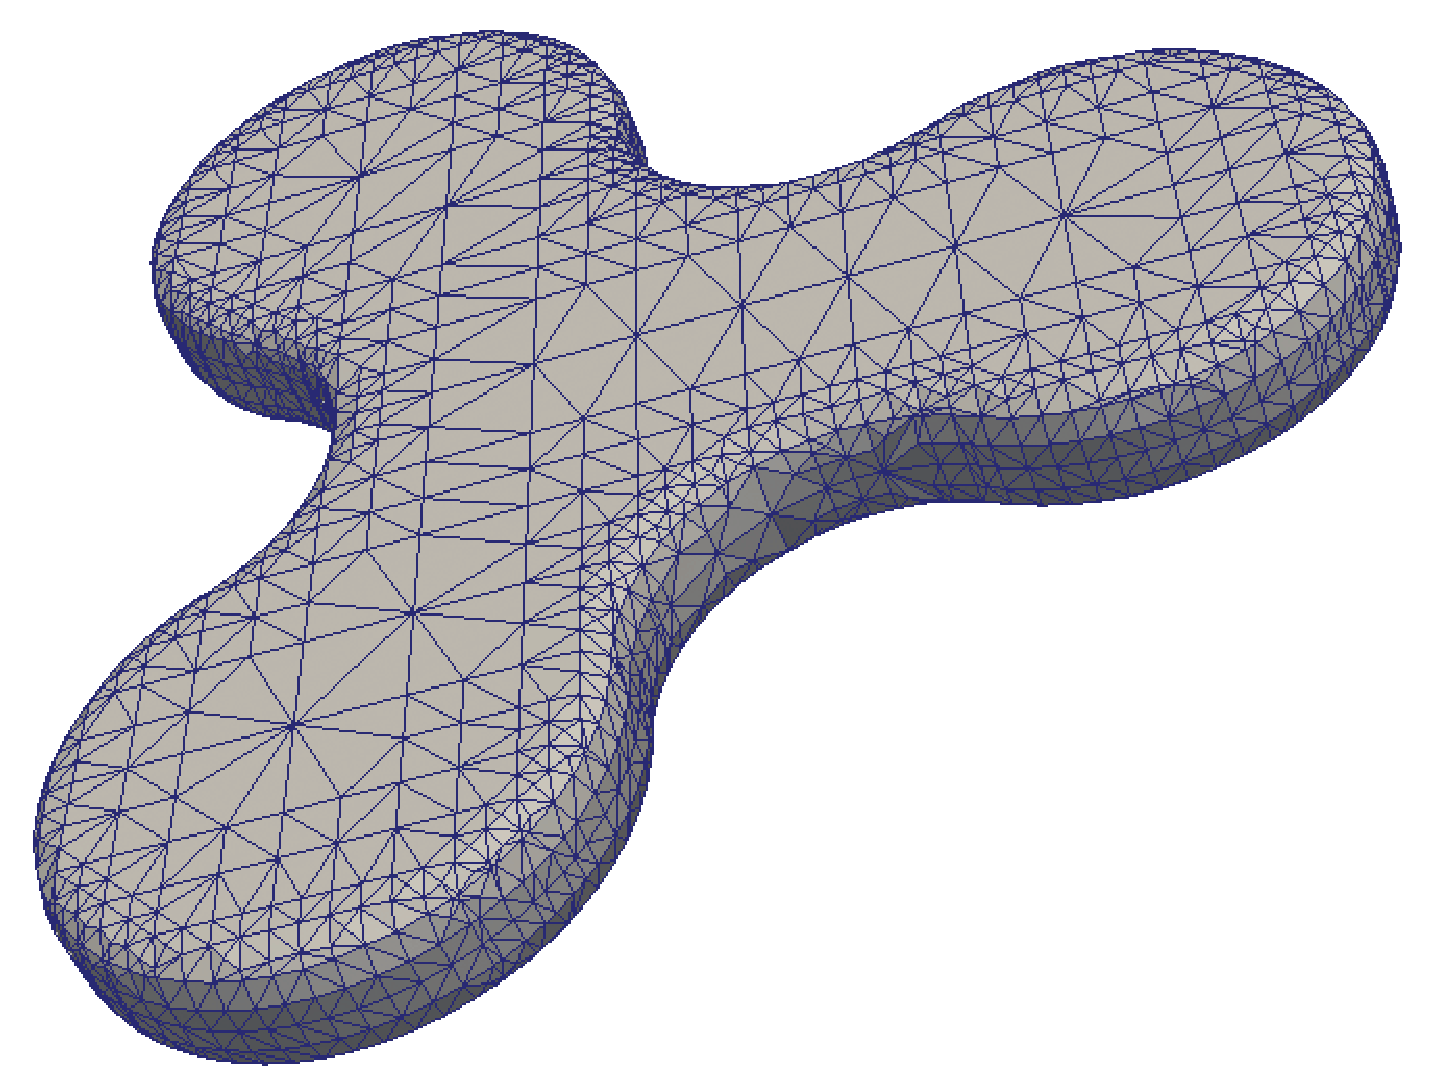
\includegraphics{octree/ex_images/spinner_full.eps}
        }
    \end{subfigure}
    \begin{subfigure}[b]{0.49\linewidth}
        \centering
        \scalebox{0.25}{
            \includegraphics{octree/ex_images/spinner_top.eps}
        }
    \end{subfigure} \\
    \begin{subfigure}[b]{0.49\linewidth}
        \centering
        \scalebox{0.25}{
            \includegraphics{octree/ex_images/spinner_side.eps}
        }
    \end{subfigure}
    \begin{subfigure}[b]{0.49\linewidth}
        \centering
        \scalebox{0.25}{
            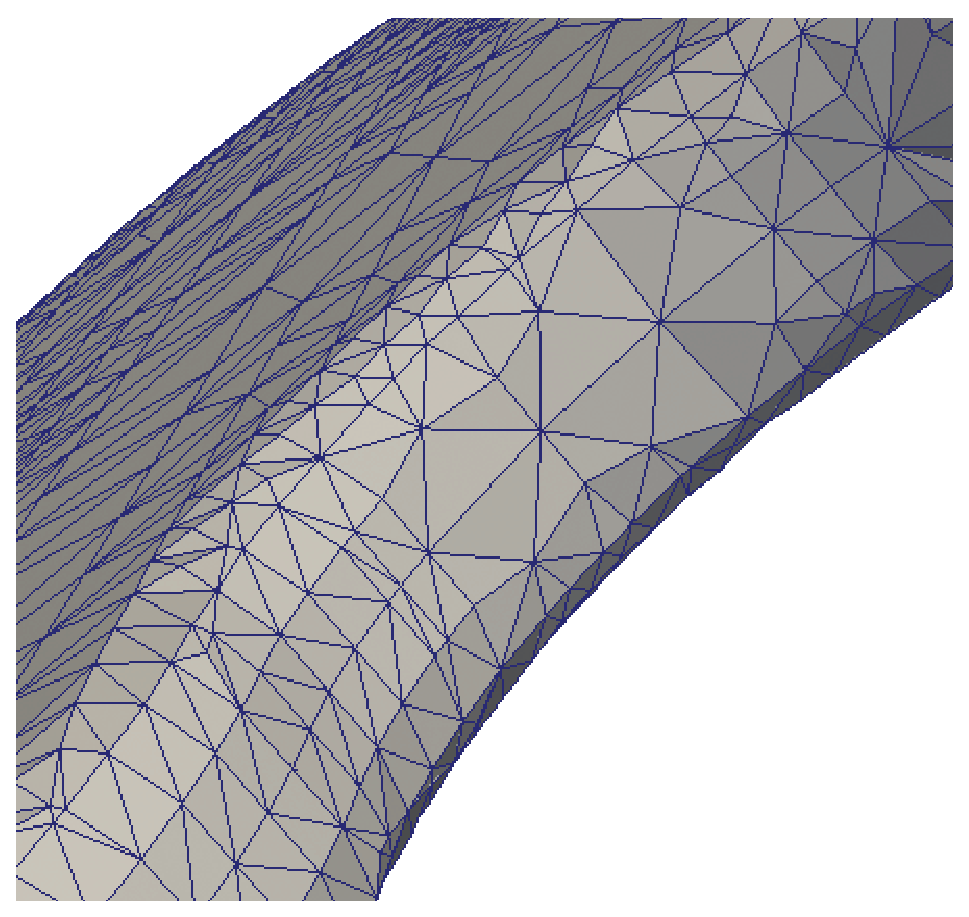
\includegraphics{octree/ex_images/spinner_part.eps}
        }
    \end{subfigure}
\end{figure}